% Template pour faire aide-mémoire
\documentclass[10pt, french]{article}

%% -----------------------------
%% Préambule
%% -----------------------------
% !TEX encoding = UTF-8 Unicode
% LaTeX Preamble
% Author : Gabriel Crépeault-Cauchon

% HOW-TO : copy-paste this file in the same directory as your .tex file, and add in your preamble the next command right after you have specified your documentclass : 
% \input{preamble-cheatsht.tex}
% ---------------------------------------------
% ---------------------------------------------

%% -----------------------------
%% Encoding packages
%% -----------------------------
\usepackage[utf8]{inputenc}
\usepackage[T1]{fontenc}
\usepackage{babel}
\usepackage{lmodern}

%% -----------------------------
%% Variable definition
%% -----------------------------


\def\cours{Mathématiques actuarielles IARD II}
\def\sigle{ACT-2008}
\def\session{Hiver 2019}
\def\auteur{Gabriel Crépeault-Cauchon // Nicholas Langevin // Alexandre Turcotte}
\def\BackgroundColor{white}
% site qui propose certaines combinaisons RGB : 
% http://latexcolor.com/
% (simplement à copier le code plus bas dans ce fichier)
\def\SectionColor{blue}
\def\SubSectionColor{blue!50!white}


%% -----------------------------
%% Margin and layout
%% -----------------------------
% Determine the margin for cheatsheet
\usepackage[landscape, hmargin=1cm, vmargin=1.7cm]{geometry}
\usepackage{multicol}

% Remove automatic indentation after section/subsection title.
\setlength{\parindent}{0cm}

% Save space in cheatsheet by removing space between align environment and normal text.
\usepackage{etoolbox}
\newcommand{\zerodisplayskips}{%
  \setlength{\abovedisplayskip}{0pt}%
  \setlength{\belowdisplayskip}{0pt}%
  \setlength{\abovedisplayshortskip}{0pt}%
  \setlength{\belowdisplayshortskip}{0pt}}
\appto{\normalsize}{\zerodisplayskips}
\appto{\small}{\zerodisplayskips}
\appto{\footnotesize}{\zerodisplayskips}

%% -----------------------------
%% URL and links
%% -----------------------------
\usepackage{hyperref}
\hypersetup{colorlinks = true, urlcolor = gray!70!white, linkcolor = black}

%% -----------------------------
%% Document policy (uncomment only one)
%% -----------------------------
%	\usepackage{concrete}
	\usepackage{mathpazo}
%	\usepackage{frcursive} %% permet d'écrire en lettres attachées
%	\usepackage{aeguill}
%	\usepackage{mathptmx}
%	\usepackage{fourier} 

%% -----------------------------
%% Math configuration
%% -----------------------------
\usepackage[fleqn]{amsmath}
\usepackage{amsthm,amssymb,latexsym,amsfonts}
\usepackage{empheq}
\usepackage{numprint}

% Mathematics shortcut
\newcommand{\reels}{\mathbb{R}}
\newcommand{\entiers}{\mathbb{Z}}
\newcommand{\naturels}{\mathbb{N}}
\newcommand{\eval}{\biggr \rvert}
\usepackage{cancel}
\newcommand{\derivee}[1]{\frac{\partial}{\partial #1}}
\newcommand{\prob}[1]{\Pr \left( #1 \right)}
\newcommand{\esp}[1]{\mathrm{E} \left[ #1 \right]}
\newcommand{\variance}[1]{\mathrm{Var} \left( #1 \right)}
\newcommand{\covar}[1]{\mathrm{Cov} \left( #1 \right)}
\newcommand{\laplace}{\mathcal{L}}

% To indicate equation number on a specific line in align environment
\newcommand\numberthis{\addtocounter{equation}{1}\tag{\theequation}}

% Actuarial notation package
\usepackage{actuarialsymbol}
\usepackage{actuarialangle}

% Matricial anotation for math symbols (\bm{•})
\usepackage{bm}
% matricial notation variable (bold style)
\newcommand{\matr}[1]{\mathbf{#1}}



%% -----------------------------
%% tcolorbox configuration
%% -----------------------------
\usepackage{tcolorbox}
\tcbuselibrary{xparse}
\tcbuselibrary{breakable}

%% Définition boite pour définition
\DeclareTColorBox{definition}{ o }% #1 parameter
{colframe=\SectionColor ,colback=\BackgroundColor , % color of the box
breakable, pad at break*=0mm, % to split the box
title = {#1},
after title = {\large \hfill \faBook}
}

%% -----------------------------
%% Graphics and pictures
%% -----------------------------
\usepackage{graphicx}
\usepackage{pict2e}

%% -----------------------------
%% insert pdf pages into document
%% -----------------------------
\usepackage{pdfpages}

%% -----------------------------
%% Color configuration
%% -----------------------------
\usepackage{color, soulutf8, colortbl}


% New color definition
% Source : http://latexcolor.com
\definecolor{burntorange}{rgb}{0.8, 0.33, 0.0}
\definecolor{burntsienna}{rgb}{0.91, 0.45, 0.32}
\definecolor{amethyst}{rgb}{0.6, 0.4, 0.8}
\definecolor{amethyst-light}{rgb}{0.6, 0.4, 0.8}

% usefull shortcut for colored text
\newcommand{\orange}{\textcolor{orange}}
\newcommand{\red}{\textcolor{red}}
\newcommand{\cyan}{\textcolor{cyan}}
\newcommand{\blue}{\textcolor{blue}}
\newcommand{\green}{\textcolor{green}}
\newcommand{\purple}{\textcolor{magenta}}
\newcommand{\yellow}{\textcolor{yellow}}


%% -----------------------------
%% Enumerate environment configuration
%% -----------------------------
% Custum enumerate & itemize Package
\usepackage{enumitem}
% French Setup for itemize function
\frenchbsetup{StandardItemLabels=true}
% Change default label for itemize
\renewcommand{\labelitemi}{\faAngleRight}

%% -----------------------------
%% Tabular column type configuration
%% -----------------------------
\newcolumntype{C}{>{$}c<{$}} % math-mode version of "c" column type
\newcolumntype{L}{>{$}l<{$}} % math-mode version of "l" column type
\newcolumntype{R}{>{$}r<{$}} % math-mode version of "r" column type
\newcolumntype{f}{>{\columncolor{green!20!white}}p{1cm}}
% configuration to force a line break within a single cell
\usepackage{makecell}



%% -----------------------------
%% Fontawesome for special symbols
%% -----------------------------
\usepackage{fontawesome}

%% -----------------------------
%% Section Font customization
%% -----------------------------
\usepackage{sectsty}
\sectionfont{\color{\SectionColor}}
\subsectionfont{\color{\SubSectionColor}}

%% -----------------------------
%% Footer/Header Customization
%% -----------------------------
\usepackage{lastpage}
\usepackage{fancyhdr}
\pagestyle{fancy}
% Header
\fancyhead{} 	% Reset
\fancyhead[L]{Aide-mémoire pour~ \cours ~(\textbf{\sigle})}
\fancyhead[R]{\auteur}

% Footer
\fancyfoot{}		% Reset
\fancyfoot[R]{\thepage ~de~ \pageref{LastPage}}
\fancyfoot[L]{\href{https://github.com/gabrielcrepeault/latex-template}{\faGithub \ gabrielcrepeault/latex-template}}

% page background color
\pagecolor{\BackgroundColor}






%% END OF PREAMBLE
% ---------------------------------------------
% ---------------------------------------------

\setlength{\abovedisplayskip}{-15pt}
\setlength{\belowdisplayskip}{0pt}
\setlength{\abovedisplayshortskip}{0pt}
\setlength{\belowdisplayshortskip}{0pt}

% Créer graphiques incluant ligne de temps pour covariance (1.8)
\usepackage{tikz}

% Créer couleur utilisée dans chapitre 2
\definecolor{ao(english)}{rgb}{0.0, 0.5, 0.0}


%% -----------------------------
%% Début du document
%% -----------------------------

\usepackage{mathrsfs}

\DeclareMathOperator*{\argmax}{arg\,max} % thin space, limits underneath in displays

%% Pour créer des trêmas avec des couleurs
\usepackage{stackengine}
\newcommand\cumlaut[2][black]{\stackon[.33ex]{#2}{\textcolor{#1}{\kern-.04ex.\kern-.2ex.}}}
%%

\begin{document}


% j'enlève le footnotesize temporairement, sinon je ne vois rien! GCC
\footnotesize % Écrire petit (peut être modifié)
\begin{multicols*}{3} % Nombre de colonnes (peut être changé plus tard.)
\section*{Rappel de Math. financière}
\subsection*{Facteurs d'actualisation}
Où les dénominateurs sont à être interprété en REGEX.
Pour exemple, pour la première c’est soit le \textcolor{cyan}{taux d'escompte} pour une une \textcolor{cyan}{annuité due} ou le taux d'intérêt pour une \textcolor{black}{immédiate}.
\begin{align*}
	\cumlaut[cyan]{a}_{\angl{n}}^{\textcolor{red}{(m)}} &= \frac{1 - v^n}{(\textcolor{cyan}{d}^{\textcolor{red}{(m)}} | i^{\textcolor{red}{(m)}})} \\
	(I^{\textcolor{blue}{(m)}}\cumlaut[cyan]{a})_{\angl{n}}^{\textcolor{red}{(m)}} &= \frac{\cumlaut[black]{a}_{\angl{n}}^{\textcolor{blue}{(m)}} - nv^n}{(\textcolor{cyan}{d}^{\textcolor{red}{(m)}} | i)} \\
	(D^{\textcolor{blue}{(m)}}\cumlaut[cyan]{a})_{\angl{n}}^{\textcolor{red}{(m)}} &= \frac{n - a_{\angl{n}}^{\textcolor{blue}{(m)}}}{(\textcolor{cyan}{d}^{\textcolor{red}{(m)}} | i)} \\
%	\ax{\angln}&= \frac{1 - v^t}{i} \\
	a_{\angl{\infty}} &= \frac{1}{i} \\
%	\ax*{\angln} &= \int_0^n v^t dt = \frac{1 - v^n}{\delta}
	d &= \frac{i}{1 + i} \\
	v &= \frac{1}{1 + i}
\end{align*}

\subsection*{Facteur d'accumulation}
\begin{align*}
\sx{\angln} &= \frac{(1+i)^{n} - 1}{i} \\
\sx**{\angln} &= \frac{(1+i)^{n} - 1}{d} \\
\end{align*}

\subsection*{Sommations}
\begin{align*}
\sum_{k = 0}^{n}r^k &= \frac{1 - r^{k + 1}}{1 - r} \\
\sum_{k = 0}^{\infty}k v^k &= \frac{v}{(1 - v)^2} \\
\sum_{k = 1}^{n}k &= \frac{n(n + 1)}{2} \\
\sum_{k = 1}^{n}k^2 &= \frac{n(n + 1)(2n + 1)}{6} \\
\end{align*}

\section{Survie et mortalité}
\setcounter{subsection}{1}
\subsection{Probabilités de survie et de décès}
\begin{itemize}
\item[$X$ : ] Âge au décès d'un nouveau-né
\item[$T_x$ : ] Durée de vie résiduelle d'un individu d'âge $x$.
\[T_x = (X-x | X \geq x) \]
\[ f_{T_x} = \px[t]{x} \mu_{x+t} \]
\[ F_{T_x}   =\qx[t]{x} = \frac{S_X(x) - S_X(x+t)}{S_X(x)}  \]
\[ \prob{t \leq T_x \leq t+u} = \qx[t|u]{x} = \px[t]{x} \cdot \qx[u]{x+t} = \qx[t + u]{x} - \qx[t]{x} \]
\[ \qx[t + y]{x} = \qx[t]{x} + \px[t]{x} \cdot \qx[y]{x + t}\]
\[S_{T_x}(t) = \exp \left\{ - \int_{0}^{t} \mu_{x+s} ds \right\} = \exp \left\{ - \int_{x}^{x + t} \mu_{s} ds \right\}  \]
\[T_x \in \mathbb{R}^+ \]

\item[$K_x$ : ] Durée de vie résiduelle entière d'un individu d'âge $x$.
\[K_x = \lfloor T_x \rfloor \]
\[\prob{K_x = k} = \prob{\lfloor T_x \rfloor = k} = \px[k|]{x} \]
\[K_x \in \mathbb{Z}^+ \]

\item[$\mu_x$ : ] Force de mortalité pour $(x)$
\[\mu_x = \frac{f_X(x)}{S_X(x)} = -\derivee{x} \Big( \ln(S_X(x)\Big) \]
\[\mu_{x+t} = - \derivee{t} \Big( \ln ( \px[t]{x}) \Big) \]
\[\alpha\mu_{x+s} + h(s) = (\px[t]{x})^\alpha e^{-\int_{0}^{t}h(s)ds } \]


\item[$R_x$ : ] Durée de vie résiduelle fractionnaire d'un individu d'âge $x$.
\[R_x = T_x - K_x\]
\[R_x \in [0, 1) \]

\item[$J^{(m)}_x$ : ] Nombre de m-ème d'années vécus durant l'année du décès.
\[J^{(m)}_x \in \{0, 1, 2, \dots, m - 1) \]
\[J^{(m)}_x= [m R_x] \]

\item[$H^{(m)}_x$ : ] Durée de vie résiduelle d'un individu d'âge $x$ exprimé en m-ème années.
\[H^{(m)}_x= [m T_x] \]
\[H^{(m)}_x \in \mathbb{Z}^+ \]


\end{itemize}

\subsection{Lois de mortalité}
\subsubsection*{Loi de Moivre}
Pas très réaliste car assume une chance \textbf{uniforme} de mourir n'importe quand alors qu'en réalité une personne agée de 90 ans a des plus grandes chances de mourir qu'un jeune de 30 ans.
 
C'est la seule loi avec un \textbf{support fini}.

\begin{align*}
	X &\sim \text{Unif}(0, \omega) \\
	S_X(x) &= 1 - \frac{x}{\omega},\: 0 \leq x \leq \omega \\
	\mu_x &= \frac{1}{\omega - x}, \: 0 \leq x \leq \omega \\
	T_x &\sim \text{Unif}(0, \omega - x) \\
	S_{T_x}(t) &= 1 - \frac{t}{\omega - x},\: 0 \leq t \leq \omega - x \\
%	K_x &\sim \text{Unif}\textit{ Discrète}(0, \omega - x - 1) \\
%	S_{K_x}(t) &= 1 - \frac{[t] + 1}{\omega - x},\: 0 \leq t \leq \omega - x - 1 \\
\end{align*}

\subsubsection*{Loi Exponentielle}
\begin{align*}
	X &\sim \mathrm{Exp}(\mu) \\
	S_x(x) &= e^{-\mu x},\: x \geq 0 \\
	T_x &\sim \mathrm{Exp}(\mu) \\
	S_{T_x}(t) &= e^{-\mu t},\: t \geq 0 \\
	T_x \sim \text{Exp}(\mu) &\Rightarrow K_x \sim \text{Géo}(p = 1 - e^{-\mu}) \\
\end{align*}

\subsubsection*{Loi de Makeham}
\begin{align*}
	X &\sim \text{Makeham}(A, B, c) \\
	A &: \text{risque d'accident} \\
	Bc^x &: \text{risque  lié au vieillissement} \\
	\mu_x &= A + B c^x,\: x \geq 0 \\
	\px[t]{x} &= e^{-At - \frac{B c^x}{ln(c)}(c^t - 1)},\: t \geq 0 \\
\end{align*}
	
\subsubsection*{Loi de Gompertz}
\begin{align*}
	X \sim \text{Makeham}(A = 0, B, c) &\Leftrightarrow X \sim \text{Gompertz}(B, c) 
\end{align*}

\subsubsection*{Loi de Weibull}
\begin{align*}
	X &\sim \text{Wei}(k, n) \\
	\mu_x &= k x^n,\; x \geq 0 \\
	\px[t]{x} &= e^{-\frac{k}{n + 1}[(x + t)^{n + 1} - x^{n + 1}]},\: t \geq 0 
\end{align*}


\subsection{Tables de mortalité}
\begin{itemize}
\item[$\ell_0$ : ] Nombre d'individus initial dans une cohorte.
\item[$\ell_x$ : ] Nombre d'invidu de la cohorte ayant survécu jusqu'à l'âge $x$.
\item[$\prescript{}{n}d_{x}$ : ] Nombre de décès entre l'âge $x$ et $x+n$.

\[\ell{x} = \sum_{y = x}^{\omega - 1} \dx{y}\]


\[\qx[t]{x} = \frac{\ell_x - \ell_{x+t}}{\ell_x}\]
\[\px[t]{x} = \frac{\ell_{x+t}}{\ell_x} \]
\[\qx[t|u]{x} = \frac{\dx[u]{x+t}}{\ell_x}\]


\end{itemize}


\subsection{Mortalité sélecte et ultime}
\begin{itemize}
\item[${[}x{]}$ : ] âge de la sélection \textit{(pas une valeur entière)}.
\item[${[}x{]} + j$ : ] âge atteint où $j$ est le temps écoulé depuis la sélection.
\item[\textbf{Période sélecte} $r$: ] Période de durée $r$ durant laquelle les effets de la sélection sont significatifs après laquelle:
\begin{align*}
	\qx{[x] + j} &= \qx{x + j} \forall j = r, r + 1, r + 2, \dots \\
	\ell_{[x] + r + j} &= \ell_{[x]} \px[r + j]{[x]} = \ell_{[x]} \px[r]{[x]} \px[j]{x + r}
\end{align*}
\end{itemize}

\subsection{Hypothèses pour les âges fractionnaires}
Pour $t \in [0,1]$ et $x \in \entiers$.

\textbf{Distribution uniforme des décès (DUD)} \\
Décès répartis uniformément sur l'année.

\begin{align*}
S_X(x + t) &= (1 - t) \times S_X(x) + t \times S_X(x + 1),  &t \in [0, 1] \\
S_X(x + t) &= \frac{(c - t)}{c} \times S_X(x) + \frac{t}{c} \times S_X(x + 1),  &t \in [0, c] \\
\end{align*}
\text{les conditions pour t et x appliquent aux 3 équations suivantes}
\begin{align*}
\qx[t]{x} &= \left(\frac{t}{c}\right) \qx[c]{x},  &t \in [0, c] \\
\mu_{x + t} &= \frac{\frac{1}{c} \qx[c]{x}}{1 - \frac{t}{c} \qx[c]{x}}, &x \in \{0, c, 2c, \dots\} \\
&\Leftrightarrow \frac{\frac{\partial}{\partial t}\qx[t]{x}}{\px[t]{x}} \\
\qx[y]{x + t} &= \frac{\left(\frac{y}{c}\right) \qx[c]{x}}{1 -\left(\frac{t}{c}\right) \qx[c]{x}}, &y \in [0, c - t] 
\end{align*}

On note que la force de mortalité à la même formule que la \\ fonction de survie car avec \textbf{DUD}, la force est uniformément \\ appliquée.

\textbf{Force constante (FC)}
\begin{align*}
S_X(x + t) &= S_X(x)^{(1 - t)} + S_X(x + 1)^t,  &t \in [0, 1] \\
S_X(x + t) &= S_X(x)^{\frac{(1 - t)}{c}} + S_X(x + 1)^{\frac{t}{c}},  &t \in [0, c] \\
\end{align*}
\begin{align*}
%\ell_{x+t} &= \ell_x^{(1-t)} \ell_{x+1}^{(t)} \\
\mu_{x + t} &= -\frac{1}{c}ln(\px[c]{x}), & t \in[0, c] \\
\qx[y]{x + t} &= 1 - (\px[c]{x})^{\frac{y}{c}}, & t \in[0, c],  y \in [0, c - t] \\
\end{align*}
% Tableau repris de Nicholas Langevin dans l'ancienne feuille de formules
\textbf{Tableau résumé lorsque} $c = 1$\\
\[
\begin{array}{|l|c|c|c|} 
                        \hline
                        & \text{DUD} & \text{FC} \\
                        \hline 
                        \actsymb[t]{q}{x} & t \cdot q_x                 & 1 - p_x^{t}   \\
                        \hline
                        \actsymb[t]{p}{x} & 1 - t \cdot q_x             & p_x^{t}   \\
                        \hline
                        \dx[1]{x}         & t \cdot \dx[n]{x}           & \lx{x} (1 - p_x^{t})  \\
                        \hline
                        f_{t_x}(t)        & q_x                         & -p_x^t  \ln(p_x)   \\
                        \hline
                        \mu_{x+t}         & \frac{q_x}{1 - t \cdot q_x} & - \ln(p_x)   \\
                        \hline
\end{array}
\]
\\
Sous: 
\begin{enumerate}
	\item[\textbf{DUD} : ] $K_x \bot R_x$
	\item[\textbf{FC} : ] $K_x \bot R_x$ ssi $p_{x + k} = p_{x} \ \forall k \in \{0, 1, ... \}$
\end{enumerate}

\subsection{Caractéristiques individuelles}

Lorsque $0 \leq x < \omega $, défini les fonctions suivantes pour 2 cas possible.

\subsubsection*{Utilisant $T_x$}
Si nous connaissons déjà la fonction de répartition/densité de $T_x$ on peut trouver:\\

\textbf{Espérance} : Espérance de la durée de vie future complète d'une personne d'âge x.
	\[	
		\esp{T_x} = 
		\eringx{x} =  
		\int_{0}^{\omega - x} t \px[t]{x} \mu_{x+t} dt = 
		\int_{0}^{\omega - x} \px[t]{x} d
	\]
\textbf{Variance}
	\begin{align*}
		V(T_x) &= 
		\int_{0}^{\omega - x} t^2 \px[t]{x} \mu_{x+t} dt = 
		\int_{0}^{\omega - x} 2 t  \px[t]{x} dt - \left(\eringx{x}\right)^2 
	\end{align*}
\textbf{Médiane} : Le nombre d'années avant que la population d'âge $x$ aujourd'hui diminue de moitié. \\
	Pour la trouver il suffit d'isoler:
	\[
		Pr[T_x \leq m(x)] = \qx[m(x)]{x} = \frac{1}{2}
	\]
\textbf{Mode} : Le moment où la population d'âge $x$ aujourd'hui connaisse le plus de décès.\\
	Pour le trouver, il faut le: 
	\[ \argmax_t \px[t]{x} \mu_{x + t} \]
	On peut uiliser la dérivée pour le trouver, mais il faut se méfier \textbf{des bornes} et que le résultat est un \textbf{maximum}.
	\[
		\derivee{t} f_{T_x}(t) = 0
	\]	

\subsubsection*{Utilisant $K_x$}
Si nous connaissons que la table de mortalité, les seules caractéristiques disponibles sont celles de $K_x$. \\
Pour obtenir celles de $T_x$ il faut poser un hypothèse pour les âges fractionnaires.\\

\textbf{Espérance} : Espérance du nombre d'années entières à vivre pour une personne d'âge x \textit{(espérance de vie abrégée)}.
	\[	
		\esp{K_x} = 
		e_{x} =  
		\sum_{k = 0}^{\omega - x - 1} k \ \qx[k | ]{x} =  
		\sum_{k = 1}^{\omega - x} \px[k]{x} 
	\]

\textbf{Variance} :  
	\begin{align*}
		V(K_x) &= 
		\sum_{k = 0}^{\omega - x - 1} k^2 \ \qx[k | ]{x} - \left(e_{x}\right)^2 
	\end{align*}

\textbf{Médiane} : Solution tel que:
	\begin{align*}
		Pr[K_x < m] &< \frac{1}{2} \\
		Pr[K_x \leq m] &\geq \frac{1}{2} 
	\end{align*}

\textbf{Mode} : 
	\[ \argmax_k \text{Pr}[K_x = k] \]


Liens entre les fonctions pour $K_x$ et $T_x$:\\
\begin{align*}
	\eringx{x} &= E[T_x] \\
	&= E[K_x] + E[R_x] \\
	&\stackrel{DUD}= e_x + \frac{1}{2} \\
	V(T_x) = &V(K_x + R_x) \\
	\stackrel{\bot}= &V(K_x) + V(R_x) \\
	\stackrel{DUD}= &V(K_x) + \frac{1}{12} \\
\end{align*}

\subsubsection*{Variables censurées}
L'espérance de vie future \textbf{d'ici} $n$ années d'un assuré d'âge $x$ (\textit{entre les âges $x$ et $x+n$}).\\

Espérance de vie \textbf{complète} temporaire \textit{n} années .
\begin{align*}
\eringx{x:\angln} &= \esp{T_x \wedge n} \\
&= \int_0^{n}t \ \px[t]{x} \mu_{x + t} dt + n \ \px[n]{x} \\
&= \int_0^{n} \px[t]{x} dt, & 0 \leq x < \omega, \\
&& 0 \leq n \leq \omega - x 
\end{align*}

Espérance de vie \textbf{abrégée} temporaire \textit{n} années.
\begin{align*}
e_{x:\angln} &= \esp{K_x \wedge n} \\
&= \sum_{k = 0}^{n - 1} k \qx[k | ]{x} + n \ \px[n]{x} \\
&= \sum_{k = 1}^{n} \px[k]{x}, & 0 \leq x < \omega - 1 \\
&& n \in \{0, 1, \dots, \omega - x - 1\} 
\end{align*}

\subsubsection*{Variables tronquées}
L'espérance de vie future \textbf{conditionnelle} au \textbf{décès} dans les $n$ prochaines années d'un assuré d'âge $x$ (\textit{entre les âges $x$ et $x+n$}).

\begin{align*}
	\esp{T_x | T_x \leq n} &= \frac{\eringx{x:\angln} - n \ \px[n]{x}}{\qx[n]{x}} \\
	\esp{K_x | K_x \leq n} &= \frac{e_{x:\angl{n + 1}} - (n + 1) \ \px[n + 1]{x}}{\qx[n + 1]{x}} \\	
	\esp{T_x | T_x \leq 1} &= a(x) = \frac{e_{x:\angl{1}} - \px{x}}{\qx{x}} \\	
\end{align*}

Lien entre espérance tronquée et censurée.
\begin{align*}
	\eringx{x:\angln} &= \esp{T_x | T_x \leq n} \qx[n]{x} + n \ \px[n]{x} \\	
		&= \esp{K_x | K_x \leq n} \qx[n + 1]{x} + (n + 1) \ \px[n + 1]{x} \\	
		&\stackrel{\bot}= e_{x:\angln} + \frac{\qx[n]{x}}{2} \\
\end{align*}

\subsubsection*{Formules de récurrence}

\begin{align*}
	\eringx{x:\angln} &= \eringx{x:\angl{m}} + \px[m]{x} \eringx{x + m:\angl{n - m}}, & 0 \leq m \leq n \leq \omega - x  \\
	e_{x:\angln} &= e_{x:\angl{m}} + \px[m]{x} e_{x + m:\angl{n - m}}, & 0 \leq m \leq n \leq \omega - x  \\
	&m, n, (\omega - x) \in \mathbb{W})
\end{align*}

\begin{align*}
	e_{x + k} &= \px{x + k} (1 + e_{x + k + 1}) \\
	\text{où } k &\in \{ (\omega - x - 2), (\omega - x - 3), \dots, 2, 1, 0  \} \\
	\text{et } e_{\omega - 1} &= 0 \ \text{comme valeur de départ}
\end{align*}

\subsection{Caractéristiques de groupe}
\begin{itemize}
%\item[$I_j(x)$ : ] Indicateur de survie du $j$\up{e} individu jusqu'à l'âge $x$.
%\[I_j(x) \sim Bin(1, S_X(x))\]
\item[$T^{(j)}$ : ] v.a. de la jème vie, $j \in \{1, \dots, \ell_a\}$
\begin{align*}
	\mathscr{L}_x &= \sum_{j = 1}^{\ell_a} I_{\{T^{(j)} > x - a\}} \\
	\Dx[n]{x} &= \sum_{j = 1}^{\ell_a} I_{\{x - a < T^{(j)}_a \le x - a + n\}} \\
\end{align*}

\item[$\mathscr{L}_x$ : ] v.a. du nombre de survivants jusqu'à l'âge $x$.
\begin{align*}
\esp{\mathscr{L}_x} &= \ell_x\\
\mathscr{L}_x &\sim \text{Bin}(\ell_0, \px[x]{0}) \\
\end{align*}
%= \sum_{j=1}^{\ell_0} I_j(x)
\item[$\prescript{}{n}{\mathcal{D}}_x$ : ] v.a. du nombre de décès entre l'âge $x$ et $x+n$.
\begin{align*}
	\esp{\Dx[n]{x}} &= \dx[n]{x} \\
	\Dx[n]{x} &\sim \text{Bin}(\ell_0, \qx[x| n]{0}) \\
	\Dx[n]{x} &= \mathscr{L}_x - \mathscr{L}_{x+n} \\
\end{align*}
\end{itemize}

On peut ensuite généraliser $\forall \ x \ge a$ 
\begin{align*}
	\mathscr{L}_x &\sim \text{Bin}(\ell_a, \px[x - a]{a}) \\
	\Dx[n]{x} &\sim \text{Bin}(\ell_a, \qx[x - a | n]{a}) \\
\end{align*}

$\text{Cov}( \Dx[n]{x}, \Dx[m]{y} )  =$
\[
	\begin{cases}
		- \qx[x - a | n]{a} \cdot \qx[y - a | m]{a}, & \color{orange}{x + n} \le\color{blue}{ y} \\
		\qx[y - a | x + n - y]{a} - \qx[x - a | n]{a} \cdot \qx[y - a | m]{a}, & \color{magenta}{y < x + n \le y + m} \\
		\qx[y - a | m]{a} - \qx[x - a | n]{a} \cdot \qx[y - a | m]{a}, & \color{violet}{y + m \le x + n} \\
	\end{cases}
\]
\\

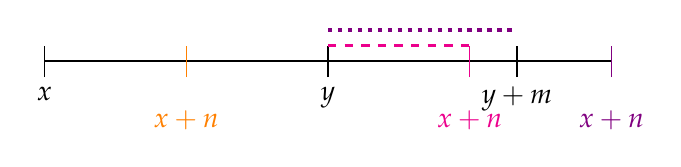
\begin{tikzpicture}[xscale=1.2]
	\draw [thick] (0,0) -- (6,0);

	\draw (0,-.2) -- (0, .2);
		\draw [orange] (1.5,-.2) -- (1.5, .2); % 1er cas
	\draw (3,-.2) -- (3, .2);
		\draw [magenta] (4.5,-.2) -- (4.5, .2); % 2ème cas
		\draw [-] [draw=magenta, dashed, very thick] (3,0.2) -- (4.5,0.2); % 2ème cas
	\draw (5,-.2) -- (5, .2);
		\draw [violet] (6,-.2) -- (6, .2); % 3ème cas
		\draw [-] [draw=violet, dotted, ultra thick] (3,0.4) -- (5,0.4); % 3ème cas
	
	\node[align=left, below] at (0,-.2)%
	{$x$};
	\node[align=left, below] at (3,-.2)%
	{$y$};
	\node[align=left, below] at (5,-.2)%
	{$y + m$};
	
	\node[align=left, below] at (1.5,-.5) %1er cas
	{\color{orange}{$x + n$}};
	\node[align=left, below] at (4.5,-.5) %2ème cas
	{\color{magenta}{$x + n$}};
	\node[align=left, below] at (6,-.5) %3ème cas
	{\color{violet}{$x + n$}};
\end{tikzpicture}

\textbf{Raccourci} pour s'en souvenir où $\ell_a$ est le nombre inital de personnes :

$\text{Cov}( \text{Groupe A}, \text{Groupe B} ) = $
\begin{align*}
	\ell_a \times \\
	\bigg( &\text{Pr}(\text{Appartenir aux groupes A et B}) \\
	&- \text{Pr}(\text{Appartenir au groupe A}) \\
	&\times \text{Pr}(\text{Appartenir au groupe B}) \bigg)
\end{align*}

\subsubsection*{Lien entre $\ell_x$ et $S_X(x)$}

\begin{align*}
	\ell_x &= \ell_a S_{T_a}(x - a) = \ell_a \ \px[x - a]{a}
\end{align*}


\section{Contrats d'assurance-vie}
Le paiement est soit en continu, soit à la fin de l'année ou à la fin de la $\frac{1}{m}$ d'année.

\subsubsection*{Notation}

${{\color{cyan}{\boxed{}}}}\text{}^{{\color{gray}{\boxed{}}}}_{{\color{brown}{\boxed{}}}}\text{}_{{\color{blue}{\boxed{}}}}^{{\color{violet}{\boxed{}}}}\prescript{}{{\color{ao(english)}{\boxed{}}}}Ax_{{\color{red}{\boxed{}}}}^{{\color{magenta}{\boxed{}}}}$

\textbf{\textcolor{red}{Couverture temporaire n années}}
\begin{itemize}
	\item[$\Ax{\termxn}$] Cas de décès.
	\item[$\Ax{\pureendowxn}$] Cas de survie.
	\item[$\Ax{x:\angln}$] Les deux cas.
	\item[$\Ax{x}$] En tout temps.
\end{itemize}

\textbf{\textcolor{brown}{Période différée}}
\begin{itemize}
	\item[$\prescript{}{m|}A_{x}$] Couverture débutant dans n années.
\end{itemize}

\textbf{\textcolor{blue}{Type de variation de la prestation}}
\begin{itemize}
	\item[$A_{x}$] Constant
	\item[$\IA{x}$] Croissant arithmétiquement
	\item[$\DA{x}$] Décroissant arithmétiquement
\end{itemize}

\textbf{{\color{violet}{Fréquence de variation}}} \\

{\color{violet}{variation m fois par année}}
\begin{align*}
	\ImA_{x} \text{ et } \DmA_{x} 
\end{align*}
{\color{violet}{\textit{(dé)}croissance continue}}
\begin{align*}
	\IbA_x \text{ et } \DbA_x 
\end{align*}

\textbf{{\color{ao(english)}{\textbf{Durée temporaire de la variation}}}}\\
$\twoletsymb{I_{\angln}}{A}_{x}$ Augmentation uniquement lors des n premières années de couverture.

\textbf{{\color{cyan}{\textbf{Prestation de base}}}}
\begin{itemize}
	\item[$b \Ax{x}$] Si quelque chose est payable c'est b.
	\item[$b \IA_x$] Paye b lorsqu'il y a décès à la \textbf{fin} de la \textit{première année} de couverture.
	\item[$b \IA_x$] Paye b lorsqu'il y a décès au \textbf{début} de la \textit{dernière année} de couverture.
\end{itemize}

\textbf{{\color{magenta}{\textbf{Moment de paiement de la prestation de décès}}}}
\begin{itemize}
	\item[$\bar{A}_x$] Au moment du décès.
	\item[$\Ax{x}^{(m)}$] À la fin de 1/m années du décès.
\end{itemize}

\textbf{{\color{gray}{\textbf{Force, ou multiple j de la, d'intérêt $\delta$}}}}

$0 \leq \delta < 1 \text{ et } j \in \mathbb{Z}_+$
\begin{itemize}
	\item[$\prescript{\delta}{}{A}_x$] Évaluation avec \textbf{force} d'intérêt $\delta$ \textit{(constante)}.
	\item[$\prescript{j}{}{A}_x$] Évaluation avec \textbf{\textit{j} fois force} d'intérêt $\delta$ \textit{(pas nécessairement constante)}.
\end{itemize}

%\subsubsection*{Principes de calcul de la prime pour un seul contrat}
%
%\begin{enumerate}
%	\item[$Z$ : ] v.a. de la valeur actualisée du montant payé selon les termees du contrat.
%\end{enumerate}
%
%Principes pour calculer la prime \textit{(unique)} à payer pour un contrat d'assurance:
%\begin{enumerate}
%	\item $\esp{Z}$ \textbf{principe d'équivalence}
%	\item $\esp{Z} + k \sigma_Z$
%	\item $\xi$ \textbf{quantile de} $Z$.\\
%\end{enumerate}
%
%Interprétations pour un seul contrat
%\begin{enumerate}
%	\item En moyenne l'assureur ne fait ni gains ni pertes
%	\item Lorsqu'il y a plusieurs contrats, le principe est équivalent au troisième mais lorsqu'il n'y en a qu'un seul alors il ne tient pas.
%	\item Plus petite prime $\pi$ telle que $Pr(Z \ge \pi) = p$
%\end{enumerate}
%
%\subsubsection*{Principes de calcul pour un portefeuille de plusieurs contrats}
%
%Suppose l'indépendance des différentes vies des contrat par défaut.
%Si une même vie achète plusieurs contrats d'assurance vie, faut tenir compte des covariances.
%
%Si contrats identiques, divise la prime totale parmis les contrats du portefeuille. 
%Si les contrats sont différents, doit trouver la surchage $\theta$ qui, lorsqu'appliqué à chacune des espérances individuelles, donnera la prime collective au total.
%
%\textbf{Surchage}: Fraction de l'espérance ajouté pour égaler la prime chargée.
%\[
%	\pi = (1 + \theta) \times \esp{Z}
%\]
%
%\textbf{Surprime}: Prime chargée en sus de l'espérance.
%
%En général lorsque $Z_j$ sont (iid):
%\begin{align*}
%	S &= \sum_{j = 1}^{n} Z_j
%\end{align*}
%
%Contrats identiques:
%\begin{enumerate}
%	\item $\esp{Z} = \pi$
%	\item $Pr(S \le n \pi) \ge p$
%\end{enumerate}
%
%Contrats non identiques \textit{la prime varie selon le type de contrat}.:
%\begin{enumerate}
%	\item $\esp{Z} = \pi$ pour chaque type de contrat
%	\item
%	\item Plus petit h t.q. $Pr(S \le h) \ge p$ avec une \textbf{surchage }égale pour tous les contrats.
%\end{enumerate}
%
%$S \sim N(\esp{S} = n \esp{Z}, V(S) = nV(Z)) $
%
%surchage et n

\subsection{Durée temporaire}

\paragraph{Assurance-vie entière} On verse le capital au décès de l'assuré

\begin{flalign*}
\Ax*{x} & = \int_{0}^{\omega - x} v^t \px[t]{x} \mu_{x+t} dt \\
\Ax{x}	& = \sum_{k=0}^{\omega - x - 1} v^{k+1} \qx[k|]{x} \\
	& = \sum_{k=0}^{\omega - x - 1} v^{k+1} \px[k]{x} \qx[]{x+k} \\
\end{flalign*}
\begin{align*}
\Ax{x} = v \qx[]{x} + v p_x \Ax{x+1}
\end{align*}


\paragraph{Assurance-vie temporaire} On verse le capital au décès de l'assuré, s'il survient dans les $n$ prochaines années.
\begin{flalign*}
\Ax*{\termxn}	& = \int_{0}^{n} v^t \px[t]{x} \mu_{x+t} dt \\
\Ax{\termxn}		& = \sum_{k=0}^{n-1} v^{k+1} \qx[k|]{x} \\
	& = \sum_{k=0}^{n-1} v^{k+1} \px[k]{x} \qx[]{x+k} \\
\end{flalign*}

\paragraph{Assurance-vie dotation pure} On verse le capital à l'assuré si celui-ci est toujours en vie après $n$ années.
\begin{align*}
\Ax{\pureendowxn}	& = \px[n]{x} v^n = \Ex[n]{x} \\
\end{align*}
où $\Ex[n]{x}$ est un facteur d'actualisation actuarielle.

\paragraph{Assurance mixte} On verse le capital à l'assuré si il décède dans les $n$ prochaines années, ou si il est toujours en vie après cette période.
\begin{align*}
\Ax*{x:\angln}	& = \int_{0}^{n} v^t \px[t]{x} \mu_{x+t} dt + v^n \px[n]{x} \\
	& = \Ax*{\termxn} + \Ax{\pureendowxn} \\
\Ax{x:\angln}		& = \sum_{k=0}^{n-1} v^{k+1} \qx[k|]{x} + v^n \px[n]{x} \\
\end{align*}

\paragraph{Assurance différée} On verse le capital à l'assuré lors de son décès seulement si le décès survient dans plus de $m$ années \footnote{Interprétation : Une assurance-vie entière qui débute dans $m$ années.}

\begin{align*}
\Ax*[m|]{x}	& = \int_{m}^{\omega -x} v^t \px[t]{x} \mu_{x+t} dt \\
	& = v^m \px[m]{x} \int_{0}^{\omega - x - m} v^t \px[t]{x+m} \mu_{(x+m)+t} dt \\
	& = \Ex[m]{x} \Ax*{x+m} \\
\Ax[m|]{x}	& = \sum_{k=m}^{\omega - x -1} v^{k+1} \qx[k|]{x} \\
	& = \sum_{k=0}^{\omega - x - m - 1} v^{k+1+m} \qx[(k+m)|]{x} \\
	& = v^m \px[m]{x} \sum_{k=0}^{\omega - (x+m) - 1} v^{k+1} \px[k]{x+m} \qx[]{x+m+k} \\
	& = \Ex[m]{x} \Ax{x+m} \\
\end{align*}
\paragraph{Lien entre assurance différée, assurance vie entière et assurance-vie temporaire}

\begin{align*}
\Ax*[m|]{x}	& = \Ax*{x} - \Ax*{\itop{x}:\angl{m}}
\end{align*}

% Je met quelques formules de increase qui permet une rapidité dans les calculs 
\paragraph{Assurance Vie entière croissante} On verse le capital au décès de l'assuré. Ce capital augmente chaque années.

\begin{align*}
	\IbA*_x &= \int_0^{\omega - x} t v^t \px[t]{x} \mu_{x+t} dt \\
		%&= \int_0^{\omega - x} \Ax*[s|]{x} ds \\ 
	\IA*_{x} &= \int_0^{\omega - x} (1 + \lfloor t \rfloor) v^t \px[t]{x} \mu_{x+t} dt \\
		&= \Ax*{x} + \Ax*[1|]{x} + \Ax*[2|]{x} + ...
\end{align*}

\paragraph{Assurance Vie temporaire croissante} On verse le capital au décès de l'assuré, s'il survient dans les $n$ prochaines années. Ce capital croit chaque années.

\begin{align*}
	\IbA*_{\termxn} &= \int_0^n t v^t \px[t]{x} \mu_{x+t} dt \\
	\IA*_{\termxn}  &= \int_0^n (1 + \lfloor t \rfloor) v^t \px[t]{x} \mu_{x+t} dt \\
		&= \actsymb{\bar{A}}{\nthtop{1}{x}:\angln} + \actsymb[1|]{\bar{A}}{\nthtop{1}{x}:\angl{n-1}} + ... + \actsymb[n-1|]{\bar{A}}{\nthtop{1}{x}:\angl1}
\end{align*}

\paragraph{Assurance vie entière croissante temporairement} On verse le capital au décès de l'assuré. Ce capital croit pendent $n$ années

\begin{align*}
	\twoletsymb{I_{\angln}}{\bar{A}}_{x}  &= \int_0^n (1 + \lfloor t \rfloor) v^t \px[t]{x} \mu_{x+t} dt \\
	& + \int_n^{\omega - x} n v^t \px[t]{x} \mu_{x+t} dt \\
		&= \Ax*{x} + \Ax*[1|]{x} + ... + \Ax*[n-1|]{x}
\end{align*}

\paragraph{Assurance Vie temporaire décroissante} On verse le capital au décès de l'assuré, s'il survient dans les $n$ prochaines années. Ce capital décroit chaque années.

\begin{align*}
	\DbA*_{\termxn} &= \int_0^{\omega - x} (n - t) v^t \px[t]{x} \mu_{x+t} dt \\
	\DA*_{\termxn}  &= \int_0^{\omega - x} (n - \lfloor t \rfloor) v^t \px[t]{x} \mu_{x+t} dt \\
		&= \actsymb{\bar{A}}{\nthtop{1}{x}:\angl1} + \actsymb{\bar{A}}{\nthtop{1}{x}:\angl2} + ... + \actsymb{\bar{A}}{\nthtop{1}{x}:\angln}
\end{align*}

\section{Contrats de rente}
\paragraph{Rente viagère} On verse une rente à l'assuré jusqu'à son décès. 
\begin{align*}
Y	&  = \ax*{\angl{T_{x}}} = \frac{1-v^{T_x}}{\delta} = \frac{1 -\overline{Z}_x}{\delta} \\
\ax*{x} & = \int_{0}^{\infty}  \ax*{\angl{T_{x}}}  \px[t]{x} \mu_{x+t} dt \\
	& = \int_{0}^{\infty} v^t \px[t]{x} dt \\
	& = \frac{1 - \Ax*{x}}{\delta} \\
\variance{Y}	& = \variance{\frac{1- v^{T_x}}{\delta}} =  \frac{\Ax*[][2]{x} - \Ax*{x}^2}{\delta^2} \\
\end{align*}

\paragraph{Rente temporaire $n$ années} Ce contrat de rentes prévoit payer une rente à l'assuré s'il est en vie, au maximum $n$ années.
\begin{align*}
Y & = \begin{cases}
\ax*{\angl{T_x}}	& , T_x < n \\
\ax*{\angln}			& , T_x \geq n \\
\end{cases} = \frac{1  - \overline{Z}_{x:\angln}}{\delta} \\
\ax*{x:\angln}	& = \int_{0}^{n} \ax*{\angl{t}} \  \px[t]{x} \  \mu_{x+t} dt \\
	& = \int_{0}^{n} v^t \px[t]{x} dt \\
	& = \frac{1 - \Ax*{x:\angln}}{\delta} \\
\variance{Y}	& = \frac{\Ax*[][2]{x:\angln} - \Ax*{x:\angln}^2}{\delta^2} \\	
 \end{align*}

\paragraph{Rente viagère différée $m$ années} C'est un contrat de rente viagère, qui débute dans $m$ années (si $(x)$ est en vie).
\begin{align*}
Y & = \begin{cases}
0											& T_x	 < 	 m	\\
v^m \ax*{\angl{T_x - m}}	& T_x 	\geq m	\\
\end{cases} = \frac{\overline{Z}_{20:\itop{\angl{10}}} - \prescript{}{m|}{\overline{Z}}_{20}}{\delta} \\ 
\ax*[m|]{x}	& = \int_{m}^{\infty} \ax*{t-m} \px[t]{x} \mu_{x+t} dt \\
	& = \Ex[m]{x} \ax*{x+m} \\
	& = \ax*{x} - \ax*{x:\angl{m}} \\
\end{align*}

\paragraph{Rente garantie (certaine) $n$ années} Le contrat prévoit une rente minimale de $n$ années, pouvant se prolonger jusqu'au décès de l'assuré.
\begin{align*}
Y & = \begin{cases}
\ax*{\angln}	& = T_x < n \\
\ax*{\angl{T_x}}	& = T_x \geq n \\
\end{cases} = \overline{Y}_{x:\angln} + \prescript{}{n|}{Y}_x \\
\ax*{\joint{x:\angln}}	& =\ax*{\angln} \cdot \qx[n]{x} + \int_{n}^{\infty} \ax*{\angl{t}} \px[t]{x} \mu_{x+t} dt \\
	& = \ax*{\angln} + \ax*[n|]{x} \\
\end{align*}

\section{Primes nivelées}
\subsection{Notation et définitions}
On définit $L$ comme la perte à l'émission d'un contrat pour l'assureur. Dans ce chapitre, le paiement de la PUN s'étalle sur une période de temps, et est conditionnel  à la survie de l'assuré. Dans le cas d'une assurance-vie,
\[L = Z - Y\]
où $Z$ est la valeur présente actuarielle est prestations à payer et $Y$ la valeur présente actuarielle des primes à recevoir. De même, pour les rentes,
\[L = Y_1 - Y_2\]
où $Y_1$ représente la valeur présente actuarielle des prestations de rente à payer et $Y_2$ la valeur présente actuarielle des primes à recevoir. \\

On définit la prime nette nivellée $\pi$ selon 3 principes. 

\subsection{Principe d'équivalence (PE)}
Sous le principe d'équivalence, $\pi^{PE}$ est la solution de
\begin{align*}
\esp{L}	& = 0 \\
\esp{Z} - \esp{Y}	& = 0 \\
\esp{Z} & = \esp{Y} \\
\end{align*}


\subsection{Principe de la perte maximale probable (PPMP)}
Sous le Principe de la perte maximale probable, $\pi^{PPMP}$ est la solution de
\begin{align*}
\prob{L < \lambda} \geq \alpha
\end{align*}
Pour résoudre, on va plutôt exprimer $\prob{L < \lambda} \leftrightarrow \px[t^*]{x}$ pour solutionner $\pi^{PPMP}$.


\subsection{Principe du portefeuille (PP)}
Similaire au PPMP, en terme de \emph{portefeuille} : $\pi^{PP}$ est la solution de
\begin{align*}
\prob{\frac{L_1 + ... + L_n}{n} < \lambda} &  \geq \alpha \\
\prob{L_1 + ... + L_n < n \lambda} & \geq \alpha \\
\end{align*}
On passe par le Théorème central limite (TCL) pour évaluer cette expression. Ainsi,
\begin{gather*}
\prob{\frac{L_1 + ... + L_n - \esp{L_1 + ... + L_n}}{\sqrt{\variance{L_1 + ... + L_n}}} < \frac{n \lambda - \esp{L_1 + ... + L_n}}{\sqrt{n \variance{L}}}  }  \geq \alpha \\
\shortintertext{Puisque les pertes à l'émission sont \emph{iid,}} \\
\prob{Z < \frac{n \lambda - n \esp{L}}{\sqrt{n \variance{L}}}}  \geq \alpha \\
\shortintertext{Par le TCL,} \\
\Phi \left( \frac{n \lambda - n \esp{L}}{\sqrt{n \variance{L}}} \right)  \geq \alpha \\
\end{gather*}
Où $Z \sim N(0,1)$ et $\Phi$ la fonction de répartition de $Z$. Le défi se trouve dans le calcul de $\variance{L}$, où
\begin{align*}
\variance{L}	& = \variance{Z - Y} \\
& = \variance{Z} + \variance{Y} - 2 \  \covar{Z, Y} \\
& = \variance{Z}  + \variance{Y} - 2 \left( \esp{ZY} - \esp{Z} \esp{Y} \right) \\
\end{align*}

\subsection{Retour de primes}
\begin{itemize}
\item Certains contrats (surtout rentes différée) vont prévoir un remboursement partiel ($\alpha$) ou total des cotisations (accumulées au taux $j < i$)\footnote{Le taux $i$ est le taux préférentiel de l'assureur, tandis que le taux $j$ est le taux offert à l'assuré pour l'accumulation de ses cotisations dans sa clause de retour de primes.} en cas de décès de l'assuré pendant la période différée.
\item On introduit la v.a. $W$, qui représente la valeur présente actuarielle d'un retour de prime, telle que
\begin{align*}
W = 
\begin{cases}
\alpha \pi v_i^{K_x + 1} \sx**{\angl{K_x + 1}j} & K_x = 0, 1, ..., n-1 \\
0	& K_x = n, n+1, ... \\
\end{cases}
\end{align*}
Alors,
\[L = Y_1 - Y_2 + W\]
\item Aussi, on trouve que
\[\esp{W} = \sum_{k=0}^{n - 1} \alpha \pi v_i^{k+1} \sx**{\angl{k+1} j} \qx[k|]{x} = \alpha \pi \psi\]
\end{itemize}

\subsection{Primes brutes}
\begin{itemize}
\item Pour tenir compte des dépenses de l'assureur, on calcule la prime \emph{brute} $G$, qui considère la valeur actualisée des dépenses de l'assureur $D$ dans le calcul de la perte à l'émission.
\item Alors, on a
\[L = Z + D - Y\]
avec $Y$ qui est fonction de $G$ (la prime brute), et non $\pi$.
\item Il y a 3 types de dépenses : 
\begin{enumerate}[label=\Roman*)]
	\item Dépenses initiales ;
	\begin{enumerate}[label=\textbullet]
		\item À l'émission du contrat ; 
		\item Commission des ventes (\% de $G$ ou du montant d'assurance $M$) ;
		\item Coût des employés qui saisissent les informations dans le système ;
		\item Impression et envoi par courrier de la police.
		\item ...
	\end{enumerate}
	\item Dépenses de renouvellement ;
	\begin{enumerate}[label=\textbullet]
		\item Commission de renouvellement (\% de $G$ ou du montant d'assurance $M$), si $G$ est payée (i.e. conditionnel à la survie de l'assuré).
	\end{enumerate}
	\item Dépenses de fin de contrat.
	\begin{enumerate}[label=\textbullet]
		\item Saisie informatique et frais de fermeture de dossier ;
		\item Émission du chèque de prestations ;
		\item Enquête (dans certains cas).
	\end{enumerate}
\end{enumerate}
\end{itemize}











\end{multicols*}
%% -----------------------------
%% Fin du document
%% -----------------------------
\end{document}